\chapter{Biên dịch front-end}
\label{Chapter3}

Toàn bộ ứng dụng front-end được xây dựng dựa trên build tool Vite, sử dụng thư viện React, kèm TypeScript. Bên cạnh đó, ứng dụng cũng sử dụng nhiều dependency liên quan, nhưng tât cả đều có thể được biên dịch nhanh dựa vào \texttt{npm}.

\section{Cài đặt các dependencies còn thiếu}
Từ thư mục gốc \texttt{salesync}, truy cập vào thư mục \texttt{front-end}.

Trong thư mục này, tiến hành gọi \texttt{npm i} để cài đặt tất cả các dependencies và packages còn thiếu.

Nếu cài đặt thành công, kết quả sẽ tương tự Hình ~\ref{figure:npm_install}.
\begin{figure}[ht]
    \centering
    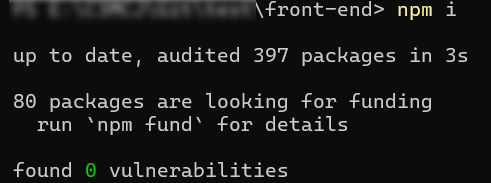
\includegraphics[width=1\linewidth]{npm_install.png}
    \caption{Cài đặt thành công các dependencies và packages}
    \label{figure:npm_install}
\end{figure}

\subsection{Tiến hành build ứng dụng}
Trong thư mục con \texttt{front-end}, tiến hành gọi \texttt{npm run build} để Vite tiến hành biên dịch toàn bộ mã nguồn React.

Nếu biên dịch thành công, một thư mục con tên \texttt{dist} sẽ được tạo, đây cũng là kết quả cuối cùng của quá trình biên dịch.